\documentclass[head_space=20.mm,foot_space=20.mm]{jlreq}
\usepackage{amsmath}
\usepackage[dvipdfmx]{graphicx}
\usepackage[dvipdfmx]{color}
\usepackage{float}
\usepackage{amsmath}
\usepackage{url}
\usepackage{siunitx}
\begin{document}
\title{タイトル}
\author{電気通信大学Ⅱ類\\カワウソ}
\date{2024年11月7日実験\\2024年11月14日提出}
%再提出日付忘れずに
\maketitle
%$d$$l_m  L_g$  $i=1i=2$


\section{目的}
あいうえお

\sectuion{テスト}
\begin{figure}[H]
  \begin{center}
  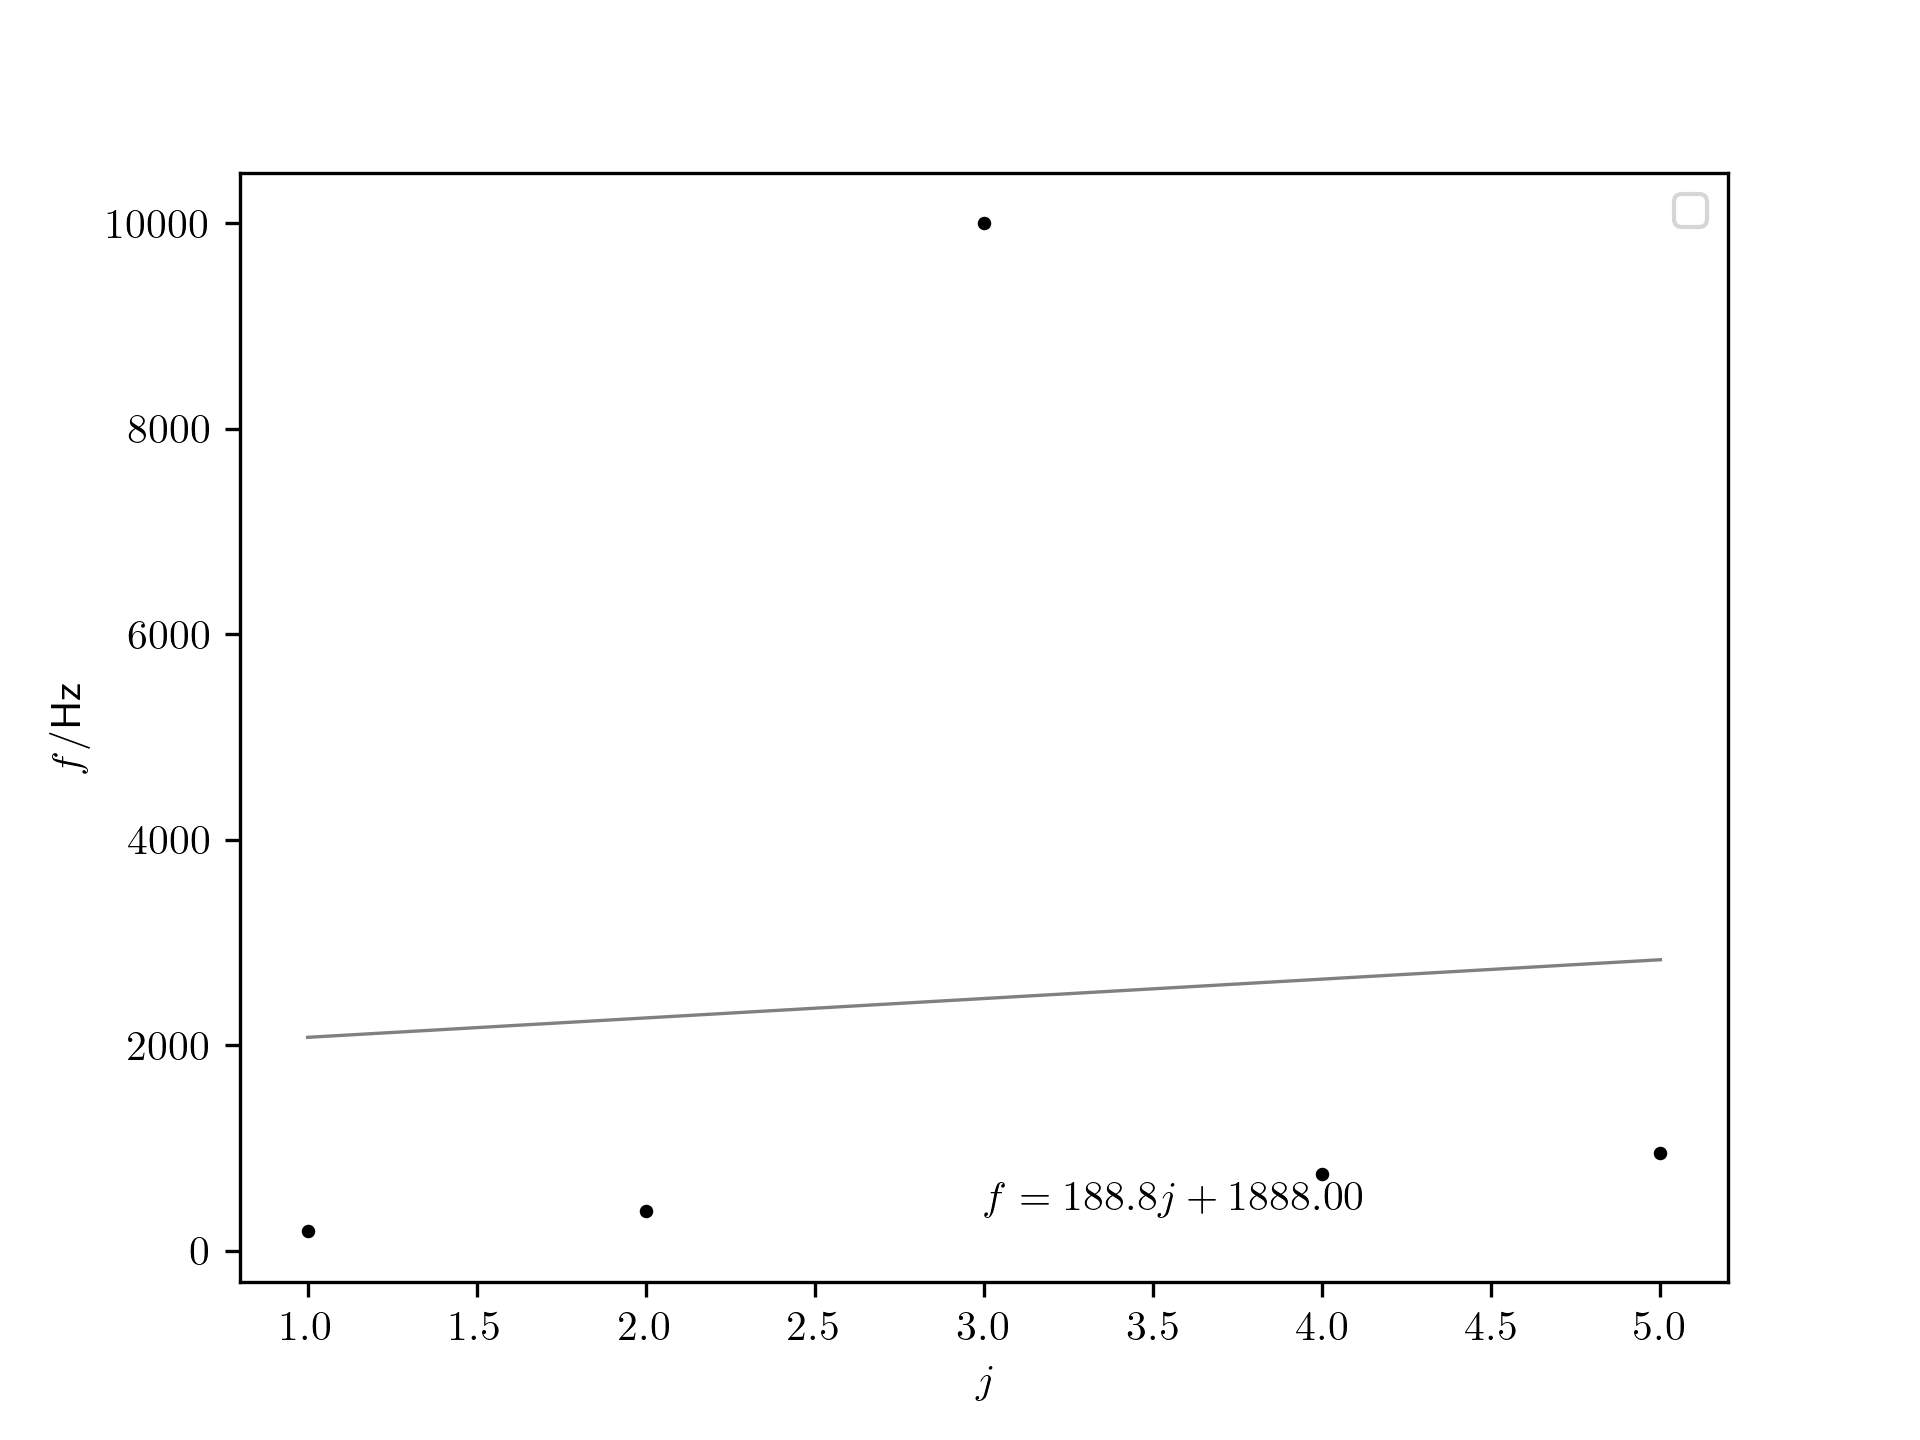
\includegraphics[width=100mm]{mokushi.png}
  \caption{直管内の気柱の振動}
  \label{fig:直管}
  \end{center}
\end{figure}
\end{document}


